\chapter{相关技术与理论基础}

\section{卷积神经网络基本原理}

卷积神经网络是一类专门用于处理具有网格结构数据（如图像）的深度神经网络。与传统全连接神经网络相比，卷积神经网络通过局部连接和权重共享机制大幅减少了参数量，更适合处理高维图像数据。

\subsection{卷积层}

卷积层是卷积神经网络的核心组件，其主要功能是自动学习输入图像的特征表示。如图\ref{fig:convolution}所示，卷积操作通过一个可学习的卷积核（也称为滤波器）在输入图像上滑动，对局部区域进行加权求和运算。

\begin{figure}[htbp]
    \centering
    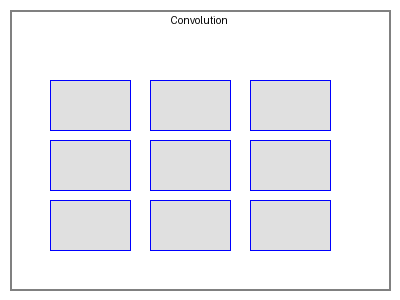
\includegraphics[width=0.7\textwidth]{assets/figures/convolution.png}
    \caption{卷积操作示意图}
    \label{fig:convolution}
\end{figure}

卷积运算的数学表达式如式\eqref{eq:conv}所示：

\begin{equation}
    y_{i,j} = \sum_{m}\sum_{n} w_{m,n} \cdot x_{i+m,j+n} + b
    \label{eq:conv}
\end{equation}

其中，$w_{m,n}$表示卷积核的权重，$b$为偏置项，$x_{i,j}$和$y_{i,j}$分别为输入和输出特征图的像素值。

卷积操作具有以下三个重要特性：

\begin{itemize}
    \item \textbf{局部连接}：每个神经元只与输入数据的局部区域相连，局部区域的大小称为感受野。这使得网络能够提取局部特征，同时减少参数量。
    \item \textbf{权重共享}：同一个卷积核在滑动过程中使用相同的权重参数。这大大减少了需要学习的参数数量，提高了网络的泛化能力。
    \item \textbf{平移不变性}：由于权重共享机制，网络对输入目标的平移、旋转等变换具有一定的不变性。
\end{itemize}

\subsection{激活函数}

激活函数为神经网络引入非线性变换，使其能够拟合复杂的非线性函数。常用的激活函数包括ReLU、Sigmoid和Tanh等。ReLU函数的表达式如式\eqref{eq:relu}所示：

\begin{equation}
    f(x) = \max(0, x)
    \label{eq:relu}
\end{equation}

ReLU函数计算简单，收敛速度快，是目前应用最广泛的激活函数。然而，ReLU神经元在训练过程中可能出现"死亡"问题，即当输入长期为负时，梯度始终为0，神经元将不再更新。

\subsection{池化层}

池化层（Pooling Layer）通过对特征图进行下采样来减少特征图的尺寸，同时保留重要的特征信息。常用的池化操作包括最大池化（Max Pooling）和平均池化（Average Pooling）。

\begin{figure}[htbp]
    \centering
    \subfloat[最大池化]{
        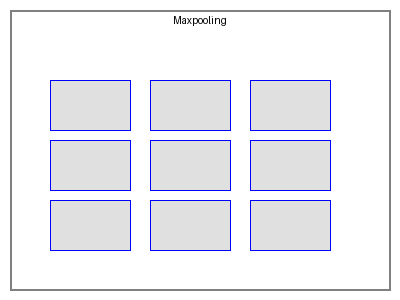
\includegraphics[width=0.45\textwidth]{assets/figures/maxpooling.png}
    }
    \subfloat[平均池化]{
        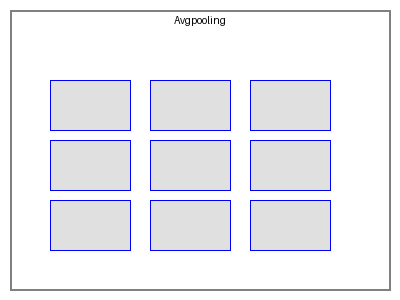
\includegraphics[width=0.45\textwidth]{assets/figures/avgpooling.png}
    }
    \caption{池化操作示意图}
    \label{fig:pooling}
\end{figure}

图\ref{fig:pooling}展示了这两种池化操作的计算过程。最大池化选择局部区域中的最大值，能够保留纹理特征；平均池化计算局部区域的平均值，使特征更加平滑。

\section{经典网络架构}

\subsection{残差网络ResNet}

随着网络层数的增加，研究者发现简单的堆叠卷积层会导致网络性能下降，这种现象称为网络退化。He等人提出的ResNet\citing{he2016deep}通过引入残差连接（Skip Connection）巧妙地解决了这一问题。

残差块的基本结构如图\ref{fig:resblock}所示。假设原始映射为$\mathcal{H}(x)$，残差映射为$\mathcal{F}(x) = \mathcal{H}(x) - x$。残差块学习的目标从直接学习$\mathcal{H}(x)$转变为学习残差$\mathcal{F}(x)$。当残差为0时，该结构相当于恒等映射，网络性能至少不会下降；当残差不为0时，网络能够学习到新的特征。

\begin{figure}[htbp]
    \centering
    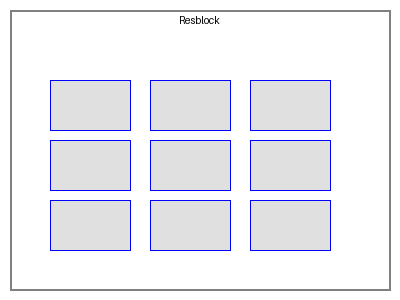
\includegraphics[width=0.5\textwidth]{assets/figures/resblock.png}
    \caption{残差块结构}
    \label{fig:resblock}
\end{figure}

残差连接的数学表达式如式\eqref{eq:residual}所示：

\begin{equation}
    y = \mathcal{F}(x, \{W_i\}) + x
    \label{eq:residual}
\end{equation}

ResNet通过堆叠多个残差块，成功训练了超过1000层的深度网络，在ImageNet数据集上将Top-5错误率降低到3.57\%。

\subsection{密集连接网络DenseNet}

Huang等人提出的DenseNet\citing{huang2017densely}采用了更为激进的连接方式——密集连接。在DenseNet中，每一层都接收所有前面层的特征图作为输入，同时将自己的特征图传递给所有后续层。

假设网络共有$L$层，密集连接可以表示为：

\begin{equation}
    x_l = H_l([x_0, x_1, \ldots, x_{l-1}])
    \label{eq:dense}
\end{equation}

其中$[x_0, x_1, \ldots, x_{l-1}]$表示前面所有层特征图的拼接，$H_l(\cdot)$表示第$l$层的非线性变换。

DenseNet的这种密集连接方式具有以下优点：加强了特征复用，减少了参数量；缓解了梯度消失问题；每层都可以直接访问损失函数的梯度，实现了隐式的深度监督。

\section{轻量化网络设计策略}

\subsection{深度可分离卷积}

深度可分离卷积（Depthwise Separable Convolution）是轻量化网络设计的核心技术，被广泛应用于MobileNet系列网络。其基本思想是将标准卷积分解为两个独立的步骤：深度卷积和逐点卷积。

标准卷积的计算量为：

\begin{equation}
    D_K \times D_K \times M \times N \times D_F \times D_F
\end{equation}

深度可分离卷积的计算量为：

\begin{equation}
    D_K \times D_K \times M \times D_F \times D_F + M \times N \times D_F \times D_F
\end{equation}

两者的计算量之比为：

\begin{equation}
    \frac{1}{N} + \frac{1}{D_K^2}
    \label{eq:dsc_ratio}
\end{equation}

当卷积核大小为$3 \times 3$时，深度可分离卷积的计算量仅为标准卷积的$\frac{1}{8}$到$\frac{1}{9}$。

\subsection{通道注意力机制}

通道注意力机制通过自适应地调整不同通道的权重，使网络能够聚焦于更重要的特征通道。SE-Net\citing{hu2018squeezeandexcitation}提出的Squeeze-and-Excitation（SE）模块是通道注意力的经典实现。

SE模块包含两个关键操作：Squeeze（压缩）和Excitation（激发）。Squeeze操作通过全局平均池化将每个通道压缩为一个标量；Excitation操作通过两个全连接层学习通道间的依赖关系。SE模块的输出如式\eqref{eq:se}所示：

\begin{equation}
    s = \sigma(W_2 \delta(W_1 y_{avg}))
    \label{eq:se}
\end{equation}

其中$\delta$为ReLU激活函数，$\sigma$为Sigmoid激活函数，$W_1$和$W_2$为两个全连接层的权重矩阵。

\section{本章小结}

本章系统介绍了卷积神经网络的基本原理，包括卷积层、激活函数和池化层等核心组件的工作机制。重点分析了ResNet和DenseNet两种经典网络架构的设计思想和创新点。最后，讨论了轻量化网络的主要设计策略，为后续章节的改进工作奠定了理论基础。
